\documentclass[12pt]{article}

\usepackage[a4paper,margin=0.5in]{geometry}

\usepackage[square,numbers,sort&compress]{natbib}
%\usepackage[sort&compress]{natbib}

\usepackage[utf8]{inputenc} % allow utf-8 input
\usepackage[T1]{fontenc}    % use 8-bit T1 fonts
\usepackage{hyperref}       % hyperlinks
\usepackage{url}            % simple URL typesetting
\usepackage{booktabs}       % professional-quality tables
\usepackage{amsfonts}       % blackboard math symbols
\usepackage{nicefrac}       % compact symbols for 1/2, etc.
\usepackage{microtype}      % microtypography
\usepackage{amsmath}
\usepackage{algorithm}
\usepackage[noend]{algpseudocode}

\usepackage{times}
\usepackage{amsfonts}
\usepackage[psamsfonts]{amssymb}
\usepackage{latexsym}
\usepackage{color}
\usepackage{graphics}
\usepackage{enumerate}
\usepackage{amstext}
\usepackage{blkarray}
\usepackage{url}
\usepackage{epsfig}
\usepackage{bm}
\usepackage{hyperref}
\hypersetup{
    colorlinks=true,
    linkcolor=blue,
    filecolor=magenta,      
    urlcolor=blue,
}
\usepackage{mathtools}


\usepackage{graphicx}
\newcommand{\bigo}[1]{{\cal O}\left(#1 \right)}
\newcommand{\p}[1]{\mathrm{P}\left(#1 \right)}
\newcommand{\vect}[1]{\mathbf{#1}}
\newcommand{\tr}{^\mathrm{t}}
\newcommand{\matr}[1]{\bm{#1}}    

\begin{document}
\thispagestyle{empty}
\begin{center}

\textbf{DS-GA 3001.001 Special Topics in Data Science: Probabilistic Time Series Analysis\\
Homework 3}
\end{center}


\noindent \textbf{Due date: Oct 25, by 6pm}\\
\noindent YG390\\

\noindent \textbf{Problem 1.} (15p)\\
Consider the HMM with K=3 latent states and discrete observations $\{1,2,3\}$, with parameters specified by:
initial distribution $\pi = [1, \, 0,\, 0]$, 
transition matrix 
$ \mathbf{A} = \begin{bmatrix}
    0 & 0.5 & 0.5\\
    1 & 0 & 0 \\
    0 & 1 & 0
    \end{bmatrix}
$, where $A_{ij} = \mathrm{P}(z_{t+1}= j | z_t= i)$ 
and likelihood $\mathrm{P}(x_t|z_t)$ described by matrix entries $B_{xz}$:
$ \mathbf{B} =  \begin{bmatrix}
    0.5 & 0.5 & 0 \\
    0.5 & 0 & 0.5 \\
    0 & 0.5 & 0.5
    \end{bmatrix}.
    $\\
 Write down all possible state sequences consistent with observations a) 1, 2, 3 and b) 1, 3, 1.\\
Let the three latent states be $\{ S_1, S_2, S_3 \}$. Given the HMM with parameters $\{A,B,\pi\}$, the model can be described as:

\begin{center}
	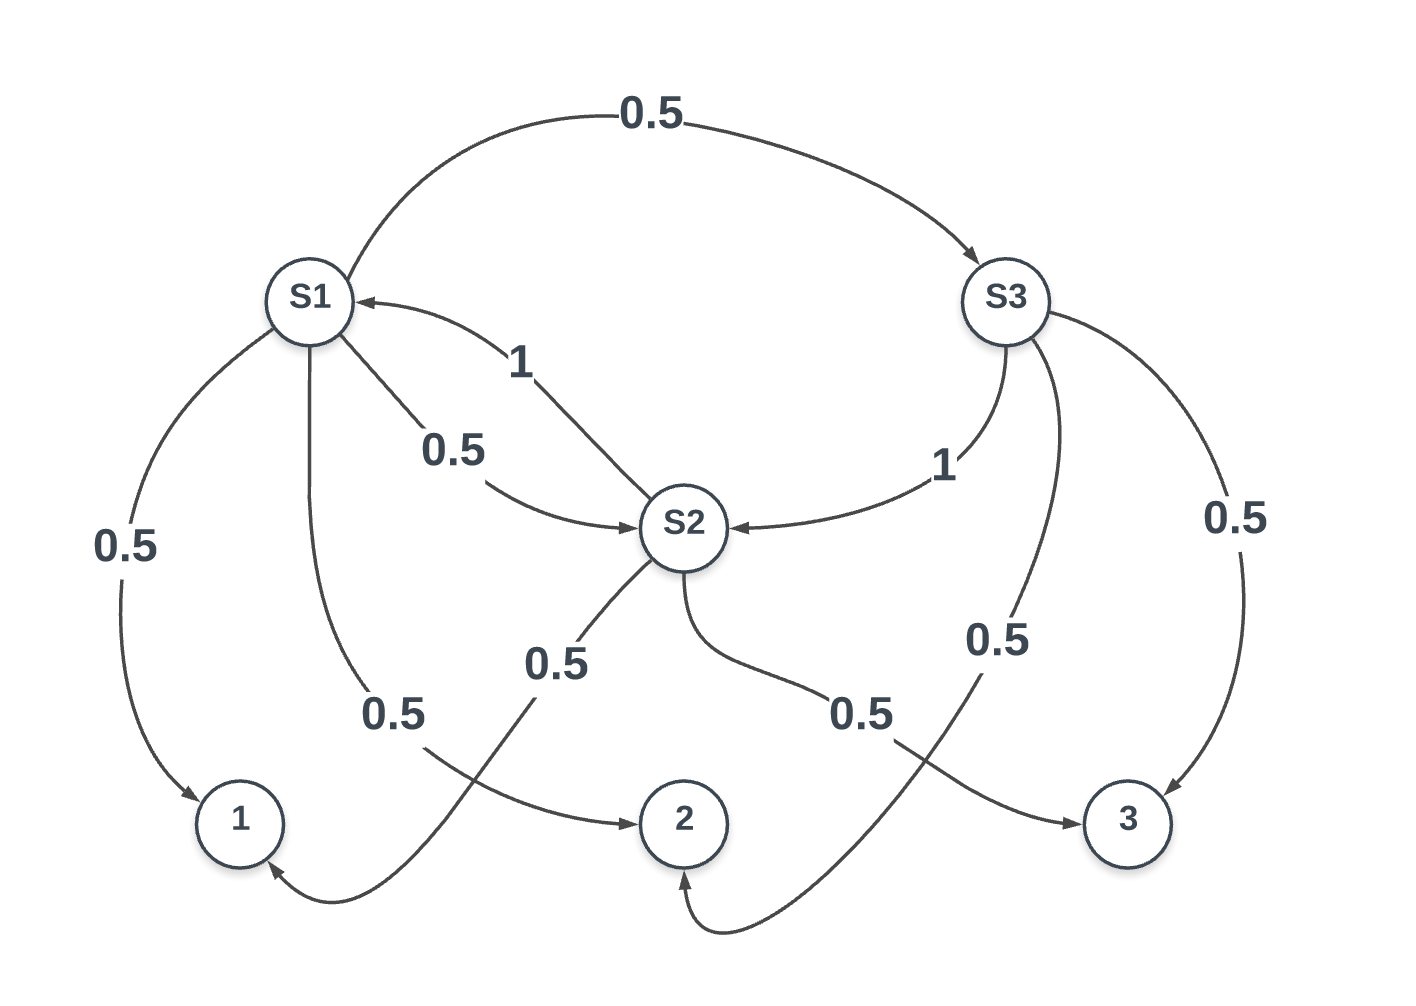
\includegraphics[width=1\linewidth]{figures/problem-1-1.png} 
\end{center}

When observing the observations 1,2, and 3 with initial distribution $\pi$ which implies we start in state $S_1$ then observing 2 means we have 0.5 probability of being in state $S_1$ or $S_3$.
However staying in state $S_1$ is not possible so the only state after seeing the sequence 1,2 is state $S_3$. Then the last observation 3 means we are in state $S_2$ or $S_3$. but from state $S_3$, 
the only existing transition is from $S_3$ to $S_2$. So the sequence of observations 1,2,3 corresponds to the state sequence $\{S_1, S_3, S_2 \}$.

When observing 1,2,1 with initial distribution $\pi$, seeing 2 after 1 implies we can be in state $S_2$ 50\% of the time or $S_3$ the rest of the time. The last observation 1 implies that the latent space is either $S_1$ or $S_2$.
Based on the transition matrix $\matr{A}$ then the only possible state sequences for the sequence of observations $\{1,2,1\}$ are $\{S_1, S_2, S_1\}$ or  $\{S_1, S_3, S_2\}$.

\noindent \textbf{Problem 2.} (15p)\\
Construct an HMM that generates the observation sequence $A^{k_1}C^{k_2}A^{k_3}C^{k_4}$ where $A^{k_1}$ denotes $k_1$ repeats of symbol $A$ and the number of repeats $k_i$ are drawn from the set $\{1,2,3\}$ with equal probability.\\

The HMM model is defined by three class of parameters $\{\matr{A}, \matr{B}, \pi \}$.
If we call $\{S_1, S_2\}$ the latent states.  For a observation sequence $A^{k_1}C^{k_2}A^{k_3}C^{k_4}$ the transition matrix $\matr{A}$ is computed so that $$a_{ij} = \frac{num\ state\ transitions\ from\ i\ to\ j}{num\ state\ transitions\ from\ i}$$
\begin{align*}
	A_{11} &= \frac{k_1 -1 + k_3 -1} {k_1-1 + k_3-1 +2} = \frac{k_1 + k_3 -2} {k_1 + k_3} \\
	A_{12} &= \frac{2}{k_1 + k_3} \\
	A_{21} &= \frac{1}{k_2-1 + 1 + k_4-1} = \frac{1} {k_2 + k_4 -1}\\
	A_{22} &= \frac{k_2-1 + k_4-1}{k_2 + k_4 -1} = \frac{k_2 + k_4 -2} {k_2 + k_4 -1}
\end{align*}

$$B_{ih}=\frac{num\ of\ times\ state\ i\ emits\ h}{num\ state\ i}$$
Since the number of repeats are drawn with equal probabilities, the emission probabilities $\matr{B}$, is the identity matrix since there are as many observations repeated for A,
then the number of state $S_1$, and the same for C and $S_2$.
$$\pi_{i}=\frac{num\ of\ chains\ start\ with\ i}{total\ num\ of\ chains}$$
We have only one chain starting with a sequence of A, which implies that we start in $S_1$ and  the initial distribution is $\pi = [1, \, 0]$.

\begin{center}
	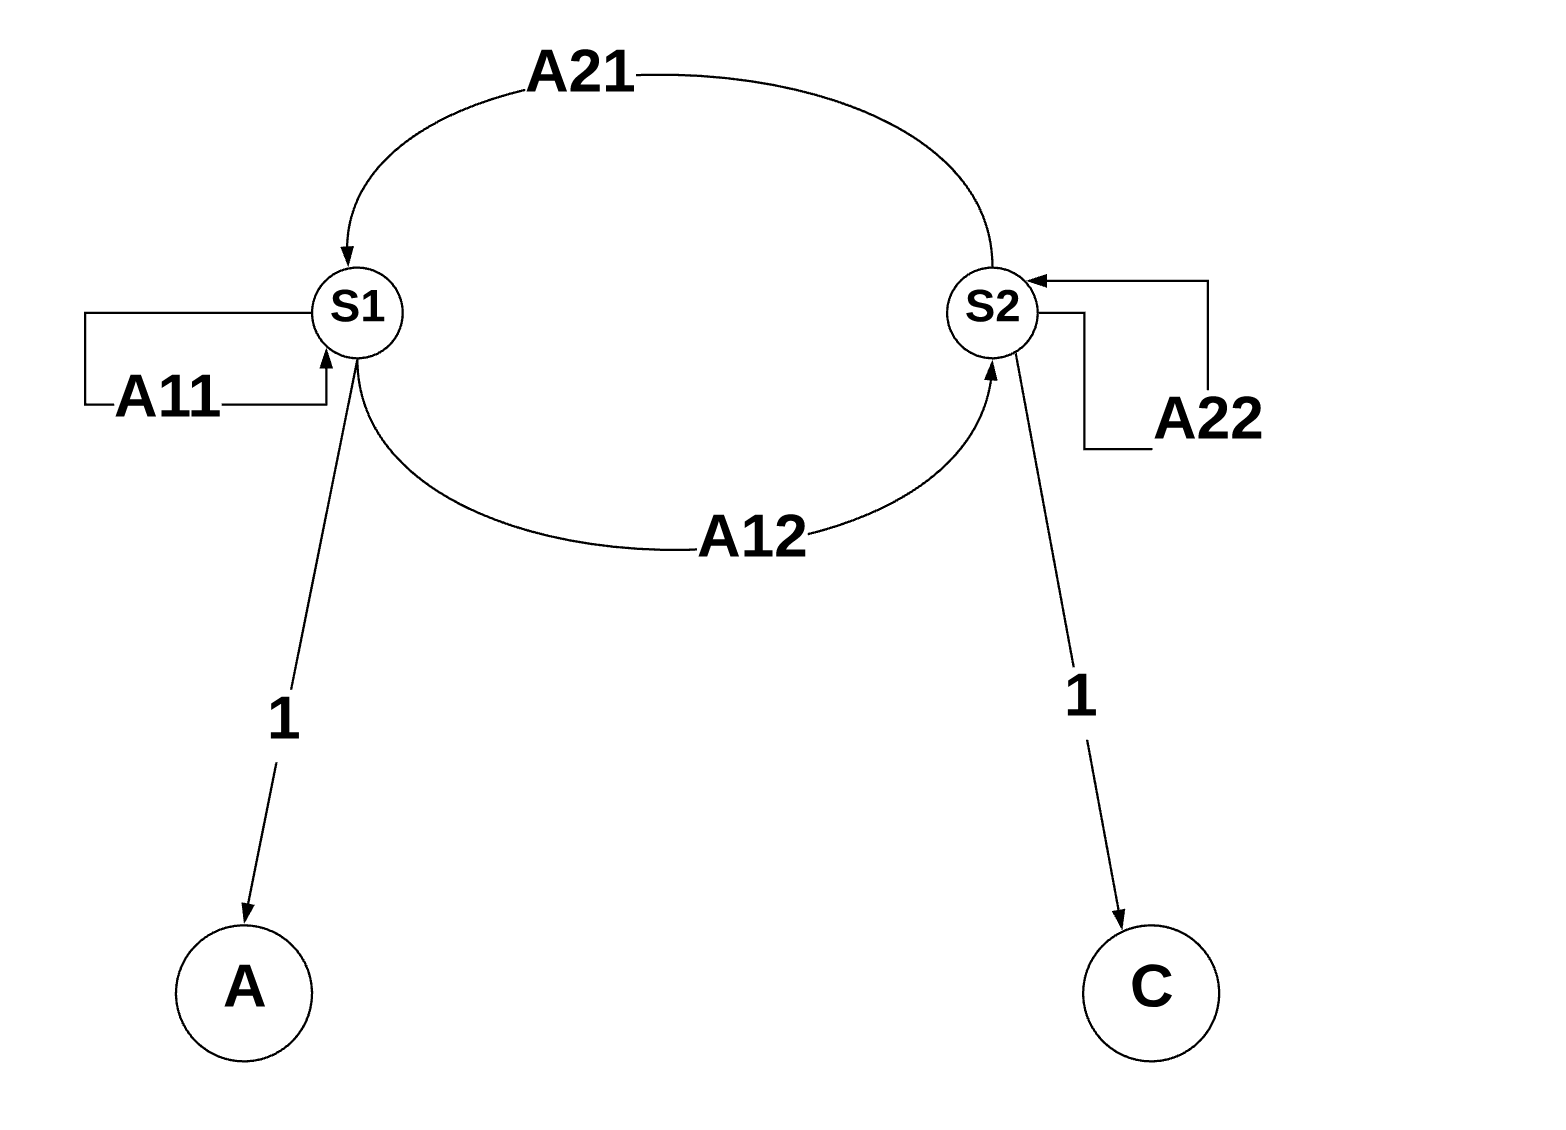
\includegraphics[width=1\linewidth]{figures/problem-2-1.png} 
\end{center}


\noindent \textbf{Problem 3.}  (20p)\\ 
Implement EM for an HMM model with K states and gaussian observations (full derivations in handout). 
Use this code to fit the weekly S\&P 500 returns data (data/sp500w.csv) for K = 2 vs. K = 3 and compare the two results. \\
Hint: Use Example 6.17 from tsa4 textbook as guideline for plots and interpretation.

\end{document}